\begin{mainquestion}{diodeconnected}{Diode-Connected NMOS Transistor}

The circuit shown below converts the MOSFET into a two-terminal device by shorting the gate and drain.

\begin{center}
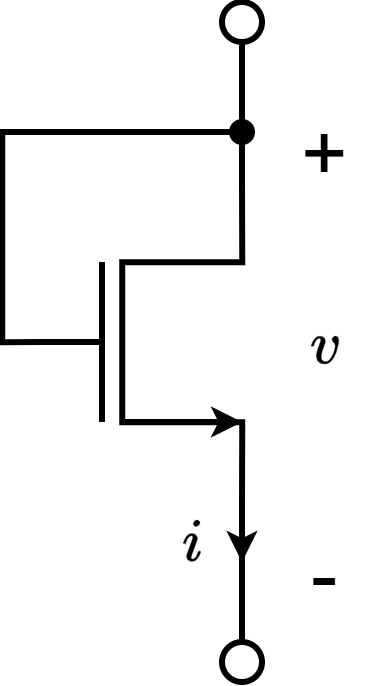
\includegraphics[height=2in]{questionbank/transistors/diode_connected/v0/circuit.png}
\end{center}

\begin{partquestion}{derive}{Derive an expression for the current versus voltage ($i$ vs. $v$) of this NMOS transistor circuit for both cutoff and non-cutoff operation. What operating regime is it in? You may assume this is an enhancement-mode transistor, {\it i.e.} $V_{tn} > 0$.}
\begin{answer}
Here, $V_{G} = V_{D}$ so $V_{GS} = V_{DS}$. Since $V_{tn} > 0$, it follows that $V_{DS} > V_{GS} - V_{tn}$. This implies that the device will always be in saturation provided $V_{GS} > V_{tn}$, or equivalently $V_{DS} > V_{tn}$. Otherwise, the device will be in cutoff where:

\[
i = 0
\]

Here, the equation for current in saturation is:

\begin{align*}
    i_D &= \frac{1}{2}k(V_{GS}-V_{tn})^2 = \frac{1}{2}k(V_{DS}-V_{tn})^2 \\
    i &= \frac{1}{2}k(v-V_{tn})^2
\end{align*}

Putting this together gives an I-V relationship:

\[
i = \left\{
  \begin{array}{ll}
    0, & v \leq V_{tn} \\
    \frac{1}{2} k \left( v - V_{tn} \right)^{2}, & v > V_{tn}
  \end{array}
\right.
\]
\end{answer}
\end{partquestion}

\begin{partquestion}{explain}{Why is this configuration called a diode-connected transistor? How does the current growth compare to that of the Shockley model?}
\begin{answer}
Like a diode, this diode-connected transistor acts as a switch at a certain applied voltage (in this case $V_{tn}$) below which the device is off and no current flows through the device. Above which, the current increases quickly as the applied voltage increases. The growth is quadratic, which is not nearly as fast as the exponential growth seen in the Shockley model of the diode.
\end{answer}
\end{partquestion}

\end{mainquestion}
